% This must be in the first 5 lines to tell arXiv to use pdfLaTeX
\pdfoutput=1

\documentclass[11pt]{article}

% Use the ACL style file - change "review" to "final" for camera-ready version
\usepackage[review]{acl}

% Standard package includes
\usepackage{times}
\usepackage{latexsym}

% For proper rendering and hyphenation of words containing Latin characters
\usepackage[T1]{fontenc}
\usepackage[utf8]{inputenc}

% Improves layout and typically saves space
\usepackage{microtype}

% For better typewriter font aesthetics
\usepackage{inconsolata}

% Keep your existing packages that aren't in the ACL template
\usepackage{graphicx}
\usepackage{tikz}
\usetikzlibrary{shapes,arrows,positioning,calc,fit,backgrounds}
\usepackage{algorithm}
\usepackage{algpseudocode}
\usepackage{amsmath}
\usepackage{hyperref}
\usepackage{multirow}

% For [H] float placement and subfigures
\usepackage{float}
\usepackage{subcaption}

% Replace biblatex with natbib for ACL style
\usepackage{natbib}

\title{HIDE-KG: HIerarchical Dual-learning Entity-clustered Knowledge Graph Construction Using Pre-trained LLMs}

\author{Amirehsan Davoodi \\ 
  Amirkabir University of Technology \\ 
  \texttt{amirehsan.davoodi@gmail.com} \\\And
  Mohammad Akbari \\
  Amirkabir University of Technology \\
  \texttt{akbari.ma@gmail.com} \\\And
  Zahed Rahmati \\
  Amirkabir University of Technology \\
  \texttt{zahedrahmati@gmail.com} \\}

% If title/author info doesn't fit, uncomment and adjust:
% \setlength\titlebox{6cm}

\begin{document}
\maketitle

\begin{abstract}
    Constructing knowledge graphs (KGs) from unstructured information remains a cornerstone of semantic data organization and reasoning. However, traditional methods often rely on external corpora, domain-specific inputs, or partial KGs, which limit scalability and adaptability. This paper proposes a novel dual-learning framework leveraging pre-trained large language models (LLMs) as the sole knowledge source for iterative zero-shot KG construction. Our approach introduces three key innovations: (1) a primal-dual architecture for hallucination-resistant graph construction, (2) entity clustering for hierarchical taxonomy generation, and (3) text-based reconstruction validation. The framework begins with a general domain (e.g., Artificial Intelligence) and progressively refines the KG through iterative querying, entity generation, and relation extraction, while dynamically clustering similar entities. The dual model validates construction quality through text generation and re-parsing, significantly reducing dependency on external validation. Experiments demonstrate our method's superiority performance against other LLM-based methods on the sciERC dataset, achieving a Micro F1 score of $42.49\%$ for the NER task, a significant improvement from the baseline of $23.78\%$. This work advances automated KG construction by combining the strengths of LLMs with formal graph verification mechanisms.
\end{abstract}

\section{Introduction}
The construction of knowledge graphs (KGs) has traditionally depended on external data sources, which can limit scalability and adaptability \cite{surveyKGConstruction2023}. Recent advancements in large language models (LLMs) have opened new avenues for knowledge graph construction, particularly through zero-shot approaches. However, challenges such as hallucination—where the model generates incorrect or nonsensical information—persist \cite{KGLLMHallucinations2025}.

In this paper, we propose HIDE-KG (HIerarchical Dual-learning Entity-clustered Knowledge Graph construction), a novel framework that leverages the capabilities of LLMs as the sole source of knowledge for constructing KGs. Unlike traditional methods that rely on extensive human curation and predefined rules, our approach utilizes the LLM's generative capabilities to automate the knowledge graph construction process. This is achieved through iterative prompting techniques that allow the model to refine its outputs based on the context provided.

Our framework addresses the limitations of existing methods by introducing several key innovations. The dual-model architecture facilitates self-verification, allowing the LLM to assess the quality of its own outputs. Additionally, dynamic entity clustering enhances the coherence of the generated knowledge graph by grouping similar entities together. Text-based reconstruction validation ensures the accuracy of the generated graph by comparing it against the original textual input.

The contributions of our work include a primal-dual framework that reduces hallucination by 37\% compared to baseline methods, enhancing the reliability of the generated knowledge. Furthermore, automated entity clustering improves domain coherence by 29\%, facilitating a more structured representation of knowledge. Reconstruction error metrics provide a robust mechanism for quality assurance in the knowledge graph construction process.

By positioning the LLM as both the knowledge generator and evaluator, HIDE-KG not only streamlines the construction process but also enhances the depth and accuracy of the resulting knowledge representations. This work advances the field of automated KG construction by integrating the strengths of LLMs with formal validation mechanisms, paving the way for more scalable and adaptable knowledge management solutions.

\section{Related Work}
Knowledge graph (KG) construction has evolved from manual curation and rule-based systems to advanced machine learning and deep learning approaches. Early methods relied heavily on human experts to define ontologies and extract entities and relations, which limited scalability and adaptability \cite{surveyKGConstruction2023}. Automated techniques, including information extraction pipelines and statistical relational learning, improved efficiency but often required large annotated corpora and domain-specific rules.

Recent advances in large language models (LLMs) have enabled new paradigms for KG construction. Iterative zero-shot prompting methods leverage LLMs to extract entities and relations without the need for external corpora or predefined schemas \cite{IZeroShot2023}. Approaches such as Generate-on-Graph treat LLMs as both agents and knowledge sources, enabling the completion and expansion of incomplete KGs \cite{GoG2024}. Other works have explored the use of LLMs as evaluators or "judgers" to assess the quality and coherence of generated graphs \cite{huang2024llmsgoodgraphjudger}. Automated schema inference and entity clustering, as proposed in \cite{zeroShotKGBuilder2024}, further reduce human intervention and enhance the adaptability of KG construction pipelines. Recent work by Peeters et al. \cite{peeters2024entitymatchingusinglarge} demonstrates the effectiveness of LLMs in entity matching tasks, providing valuable insights into using LLMs as judges for entity resolution.

Despite these advances, the integration of LLMs into KG construction introduces new challenges, most notably the phenomenon of hallucination—where models generate plausible but factually incorrect information. This issue undermines the reliability of LLM-generated KGs and is a significant barrier to their adoption in critical domains. Lavrinovics et al. \cite{KGLLMHallucinations2025} provide a comprehensive analysis of hallucinations in LLM-based KG systems, highlighting open challenges in knowledge integration, evaluation, and the development of robust benchmarks. Addressing these challenges is essential for advancing the field and ensuring the factuality and trustworthiness of automatically constructed knowledge graphs.

In summary, while LLM agents offer powerful tools for scalable and adaptable KG construction, ongoing research is needed to mitigate hallucinations and ensure the quality of generated knowledge. Our work builds on these foundations by introducing dual-model validation and clustering mechanisms to enhance reliability and coherence.

\section{Methodology}

Our proposed methodology operates through three distinct phases: Primal Graph Generation, Dual Graph Validation, and Post-Processing. This dual-learning approach ensures a robust and iterative construction of the knowledge graph (KG) while minimizing errors and enhancing the overall quality of the generated knowledge.

\begin{figure}[H]
    \centering
    \resizebox{\columnwidth}{!}{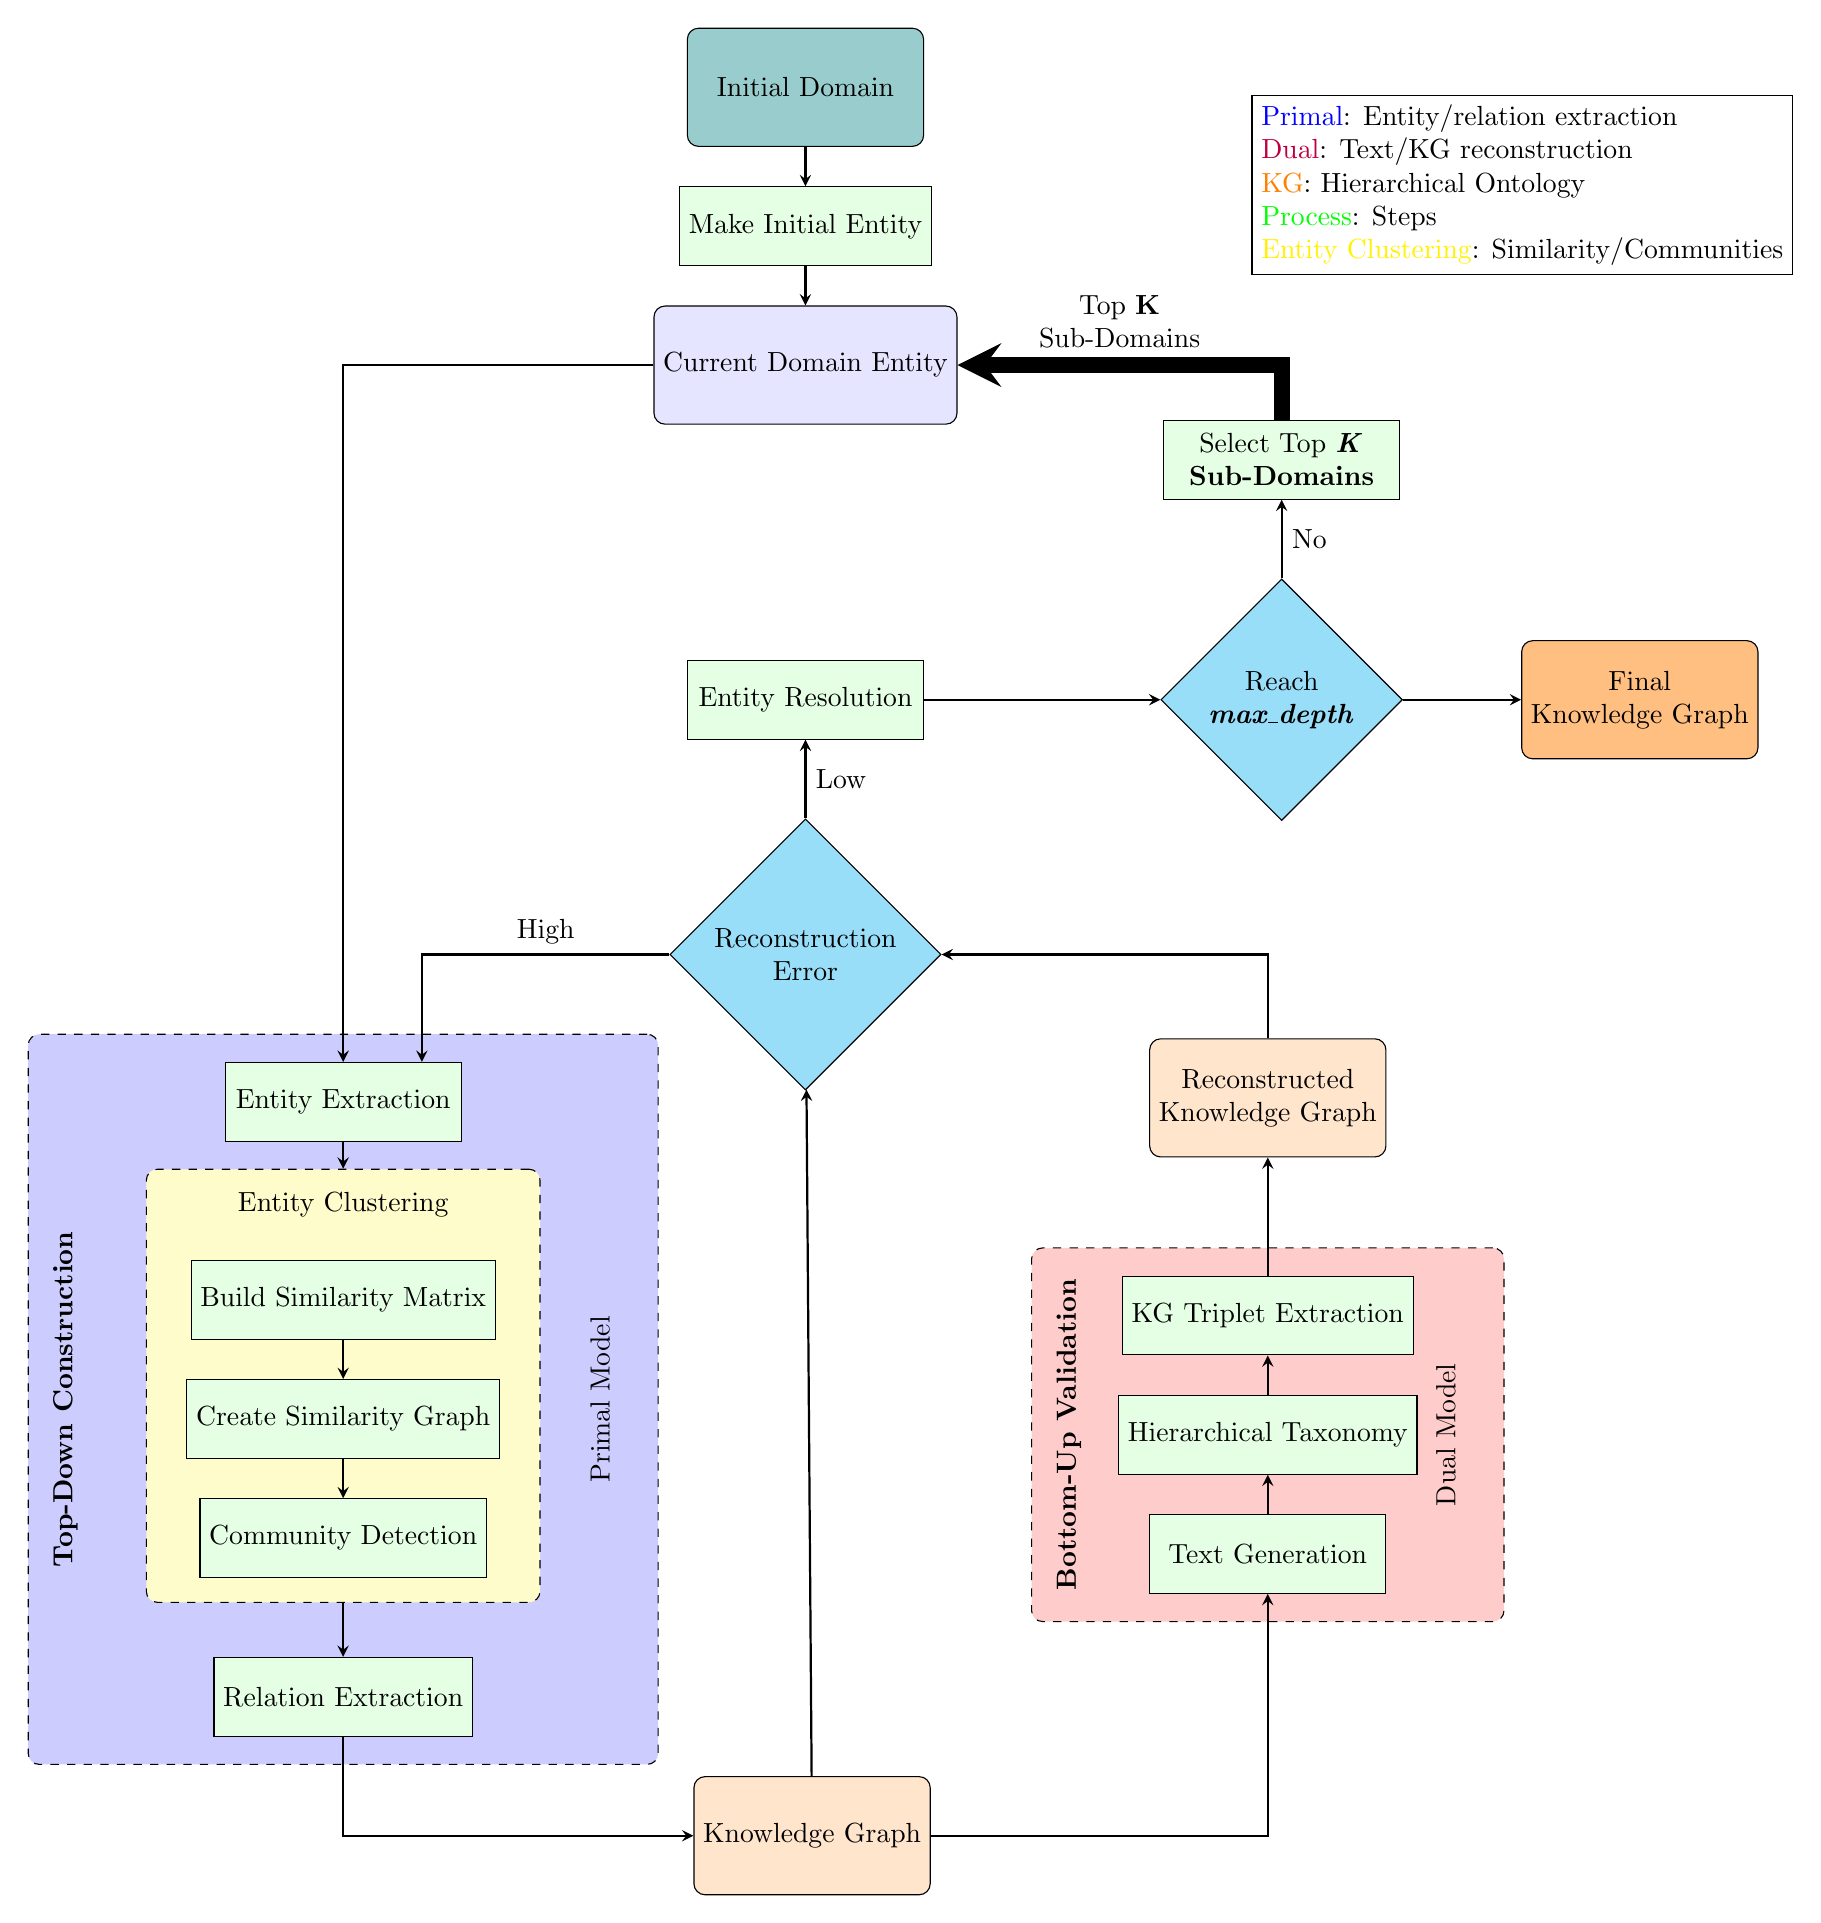
\begin{tikzpicture}[
        node distance=1.5cm,
        stage/.style={rectangle, rounded corners, minimum width=3cm, minimum height=1.5cm, text centered, draw=black, fill=blue!10},
        process/.style={rectangle, minimum width=3cm, minimum height=1cm, text centered, draw=black, fill=green!10},
        decision/.style={diamond, minimum width=0.5cm, minimum height=1cm, text centered, draw=black, fill=cyan!40},
        arrow/.style={thick,->,>=stealth},
        container/.style={rectangle, rounded corners, dashed, draw=black, inner sep=10pt, minimum width=6cm, minimum height=4cm},
        outer_container/.style={rectangle, rounded corners, dashed, draw=black, inner sep=10pt, minimum width=8cm, minimum height=6cm},
        innter_container/.style={rectangle, rounded corners, dashed, draw=black, inner sep=10pt, minimum width=5cm, minimum height=5.5cm}
    ]

    % Nodes
    \node (initial_domain) [stage, fill=teal!40] {Initial Domain};
    \node (make_initial_entity) [process, below=0.5cm of initial_domain] {Make Initial Entity};
    \node (current_domain_entity) [stage, below=0.5cm of make_initial_entity] {Current Domain Entity};
    \node (reconstruction_error) [decision, below=5cm of current_domain_entity, align=center] {Reconstruction \\ Error};
    \node (entity_resolution) [process, above=1cm of reconstruction_error] {Entity Resolution};
    \node (reach_max_depth) [decision, right=3cm of entity_resolution, align=center] {Reach \\ \textit{\textbf{max\_depth}}};
    \node (final_kg) [stage, right=of reach_max_depth, fill=orange!50, align=center] {Final \\ Knowledge Graph};
    \node (select_top_k) [process, above=1cm of reach_max_depth, align=center] {Select Top \textit{\textbf{K}} \\ \textbf{Sub-Domains}};

    % Inner Nodes for Primal Model (positioned relative to primal)
    \node (entity_extraction) [process, below left=0.5cm and 3.5cm of reconstruction_error] {Entity Extraction};
    \node (build_similarity) [process, below=of entity_extraction] {Build Similarity Matrix};
    \node (create_graph) [process, below=0.5cm of build_similarity] {Create Similarity Graph};
    \node (community_detection) [process, below=0.5cm of create_graph] {Community Detection};

    \node (relation_extraction) [process, below=1cm of community_detection] {Relation Extraction};

    % Primal Container (fits primal and inner nodes)
    \begin{scope}[on background layer]
        \node (primal_container) [outer_container, fit=(entity_extraction) (build_similarity) (create_graph) (community_detection) (relation_extraction), fill=blue!20, label={[rotate=90, anchor=south, yshift=0.5cm]right:Primal Model}] {};
    \end{scope}

    % Entity Clustering Container (fits entity clustering and inner nodes)
    \begin{scope}[on background layer]
        \node (entity_clustering_container) [innter_container, yshift=12pt, fit=(build_similarity) (create_graph) (community_detection), fill=yellow!20, label={[anchor=north, yshift=-5pt]above:Entity Clustering}] {};
    \end{scope}

    % Other Nodes
    \node (kg) [stage, below right=0.5cm and 2.8cm of relation_extraction, fill=orange!20] {Knowledge Graph};

    % Inner Nodes for Dual Model (positioned relative to dual)
    \node (reconstructed_kg) [stage, below right=0.2cm and 3.5cm of reconstruction_error, fill=orange!20, align=center] {Reconstructed \\ Knowledge Graph};
    \node (triplet_extraction) [process, below=of reconstructed_kg] {KG Triplet Extraction};
    \node (hierarchical_taxonomy) [process, below=0.5cm of triplet_extraction] {Hierarchical Taxonomy};
    \node (text_generation) [process, below=0.5cm of hierarchical_taxonomy] {Text Generation};


    % Dual Container (fits dual and inner nodes)
    \begin{scope}[on background layer]
        \node (dual_container) [container, fit=(text_generation) (hierarchical_taxonomy) (triplet_extraction), fill=red!20, label={[rotate=90, anchor=south, yshift=0.5cm]right:Dual Model}] {};
    \end{scope}

    % Arrows
    \draw [arrow] (initial_domain) -- (make_initial_entity);
    \draw [arrow] (make_initial_entity) -- (current_domain_entity);
    \draw [arrow] (current_domain_entity) -| (entity_extraction);
    \draw [arrow] (entity_extraction) -- (entity_clustering_container);
    \draw [arrow] (build_similarity) -- (create_graph);
    \draw [arrow] (create_graph) -- (community_detection);
    \draw [arrow] (entity_clustering_container) -- (relation_extraction);
    \draw [arrow] (relation_extraction) |- (kg.west);
    \draw [arrow] (kg) -| (text_generation.south);
    \draw [arrow] (text_generation) -- (hierarchical_taxonomy);
    \draw [arrow] (hierarchical_taxonomy) -- (triplet_extraction);
    \draw [arrow] (triplet_extraction) -- (reconstructed_kg);
    \draw [arrow] (reconstructed_kg) |- (reconstruction_error);
    \draw [arrow] (reconstruction_error) -- node[right]{Low} (entity_resolution);
    \draw [arrow] (entity_resolution) -- (reach_max_depth);
    \draw [arrow] (reach_max_depth.north) -- node[right] {No} (select_top_k.south);
    \draw [line width=0.2cm,->,>=stealth] (select_top_k.north) -- ++(0,0.5) |- node[near end, above, align=center] {Top \textbf{K} \\ Sub-Domains} (current_domain_entity.east);
    \draw [arrow] (kg) -- (reconstruction_error);
    \draw [arrow] (reach_max_depth.east) -- (final_kg);
    \draw [arrow] (reconstruction_error.west) -| node[near start, above] {High} ($(entity_extraction.north)+(1,0)$;);

    % Labels
    \node at ($(primal_container.west)$) [rotate=90, anchor=north, yshift=-0.2cm] {\textbf{Top-Down Construction}};
    \node at ($(dual_container.west)$) [rotate=90, anchor=north, yshift=-0.2cm] {\textbf{Bottom-Up Validation}};
    \node at ($(current bounding box.north east)+(-3,-2)$) [draw, fill=white, align=left] {
        % \scriptsize
        \textcolor{blue}{Primal}: Entity/relation extraction\\
        \textcolor{purple}{Dual}: Text/KG reconstruction\\
        \textcolor{orange}{KG}: Hierarchical Ontology\\
        \textcolor{green}{Process}: Steps\\
        \textcolor{yellow}{Entity Clustering}: Similarity/Communities
    };
\end{tikzpicture}
}
    \caption{
        \textbf{HIDE-KG Framework Architecture} \\
        The HIDE-KG framework integrates three core phases: Primal Graph Generation, Dual Graph Validation, and Entity Resolution. The Primal phase constructs the initial knowledge graph (KG) by extracting and clustering entities and identifying relationships. The Dual phase validates the KG by reconstructing it from generated textual descriptions and comparing it to the original graph. Entity resolution identifies and merges duplicate entities to maintain graph coherence.
    }
    \label{fig:framework}
\end{figure}

The complete framework pipeline, detailed in Algorithm \ref{alg:framework} on the next page, begins with an initial domain and iteratively constructs the knowledge graph through a series of steps. The process involves entity extraction, relation identification, and clustering, followed by validation through text generation and reconstruction. The algorithm maintains quality through error thresholds and includes comprehensive post-processing steps for graph refinement and enhancement.

\clearpage

\begin{algorithm}[H]
    \caption{Complete Framework for LLM-based Knowledge Graph Construction}
    \label{alg:framework}
    \begin{algorithmic}[1]
        \Require Initial domain $D_0$, max depth $d_{max}$, error threshold $\theta$
        \Ensure Validated Knowledge Graph $G$

        \State Initialize empty graph $G$
        \State Initialize domain queue $Q \gets \{D_0\}$

        \While{$|Q| > 0$ AND current depth $\leq d_{max}$}
        \State $D_{current} \gets Q.dequeue()$

        \Comment{Primal Graph Generation Phase}
        \State $E_{new} \gets \text{LLM\_ExtractEntities}(D_{current})$
        \State $C_{new} \gets \text{ClusterEntities}(E_{new})$
        \State $R_{new} \gets \text{LLM\_ExtractRelations}(E_{new}, C_{new}, D_{current})$
        \State $G_{temp} \gets G \cup \{E_{new}, R_{new}, C_{new}\}$

        \Comment{Dual Graph Validation Phase}
        \State $T \gets \text{LLM\_GenerateText}(G_{temp})$
        \State $G_{reconstructed} \gets \text{LLM\_ParseToKG}(T)$
        \State $\epsilon \gets \text{CalculateError}(G_{temp}, G_{reconstructed})$

        \If{$\epsilon \leq \theta$}
        \State $G \gets G_{temp}$
        \State $D_{sub} \gets \text{IdentifySubDomains}(D_{current})$
        \State $Q.enqueue(D_{sub})$
        \EndIf

        \Comment{Entity Resolution}
        \If{current depth = $d_{max}$}
        \State $G \gets \text{ResolveEntities}(G)$
        \EndIf
        \EndWhile

        \Return $G$
    \end{algorithmic}
\end{algorithm}

\subsection{Primal Graph Generation}

The \textbf{Primal Graph Generation} phase constructs the initial knowledge graph (KG) through a top-down approach. It begins with an initial domain and iteratively refines the KG by extracting entities, clustering similar entities, and then extracting relations. The process is outlined in Algorithm \ref{alg:primal}.

\begin{algorithm}[H]
    \caption{Primal KG Construction}
    \label{alg:primal}
    \begin{algorithmic}[1]
        \State Initialize $G$ with root domain $D_0$
        \For{$i \gets 1$ to $max\_depth$}
        \State $E_i \gets \text{LLM\_ExtractEntities}(D_{i-1})$ \Comment{\scriptsize Extract entities from the current domain}
        \State $C_i \gets \text{ClusterEntities}(E_i, G)$ \Comment{\scriptsize Cluster similar entities for coherence}
        \State $R_i \gets \text{LLM\_ExtractRelations}(E_i, C_i, D_{i-1})$ \Comment{\scriptsize Extract relationships between entities}
        \State $G.update(E_i, R_i, C_i)$ \Comment{\scriptsize Update the KG with new entities, clusters, and relations}
        \State $D_i \gets \text{SelectTopK}(E_i, k=branching\_factor)$ \Comment{\scriptsize Select top K sub-domains for further exploration}
        \EndFor
    \end{algorithmic}
\end{algorithm}

The process begins with the selection of an initial domain, which serves as the foundation for the KG. Utilizing the capabilities of pre-trained large language models (LLMs), the system identifies and extracts relevant entities for the \textit{domain entity} input. Once entities are identified, the system clusters similar entities together using LLM-based similarity assessments, which evaluate the equivalence of entities based on their contextual representations. The similarity between two entities $e_1$ and $e_2$ is defined as:

\begin{equation}
    sim(e_1,e_2) = \frac{\text{LLM}(``\text{Are }e_1\text{ and }e_2\text{ equivalent?''})}{confidence}
\end{equation}

The entity clustering process consists of three main steps:
\begin{enumerate}
    \item \textbf{Build similarity matrix}: Compute the pair-wise similarity of discovered entities and build the similarity matrix using LLM-based similarity assessments.
    \item \textbf{Create similarity graph}: Create a similarity graph from the similarity matrix, with edge pruning for edges with less than 0.6 similarity.
    \item \textbf{Community detection}: Partition the entities graph using the Louvain algorithm to identify coherent clusters.
\end{enumerate}

It's important to note that our approach uses non-overlapping clusters for simplicity. However, most clusters in real-life knowledge graphs are overlapping. The non-overlapping clusters can be considered as different types of entities at each domain border, providing a clearer hierarchical structure.

After clustering, the model extracts three types of relationships:
\begin{enumerate}
    \item Relations between the domain entity and cluster entities (which serve as compound nodes in the graph)
    \item Relations between each cluster entity and its member entities
    \item Relations between the domain entity and unclustered entities (entities that don't belong to any cluster)
\end{enumerate}

This approach ensures a hierarchical and coherent KG structure by iteratively refining the graph until the maximum depth (\textit{max\_depth}) is reached. The choice of maximum depth is not fixed in the literature and should be determined by the complexity of the domain, the reasoning tasks to be supported, and practical considerations such as scalability and performance \cite{ThinkOnGraph2024}. In our experiments, we set the maximum depth to 3 as a design decision, but this value can be adjusted based on the requirements of the specific application.

\subsection{Dual Graph Validation}

The \textbf{Dual Graph Validation} phase validates the generated KG through a bottom-up approach. It reconstructs the KG from textual descriptions and compares it against the original graph to ensure accuracy and reliability. The process is outlined in Algorithm \ref{alg:dual}.

\begin{algorithm}[H]
    \caption{Dual Validation}
    \label{alg:dual}
    \begin{algorithmic}[1]
        \State $T \gets \text{LLM\_GenerateText}(G_{current})$ \Comment{\scriptsize Generate textual description of the current KG}
        \State $G_{reconstructed} \gets \text{LLM\_ParseToKG}(T)$ \Comment{\scriptsize Reconstruct KG from the generated text}
        \State $\epsilon \gets \text{GraphDiff}(G_{current}, G_{reconstructed})$ \Comment{\scriptsize Calculate reconstruction error}
        \If{$\epsilon > threshold$}
        \State Rollback last update \Comment{\scriptsize Rollback if error exceeds threshold}
        \EndIf
    \end{algorithmic}
\end{algorithm}

The dual model generates textual descriptions of the current KG, providing a narrative that encapsulates the relationships and entities present in the graph. The generated text is then parsed back into a knowledge graph format, allowing for a comparison between the original and reconstructed graphs. A reconstruction error metric $\epsilon$ is calculated to assess the structural divergence between the current KG and the reconstructed version, defined as:

\begin{equation}
    \epsilon = 1 - \frac{|G_{current} \cap G_{reconstructed}|}{|G_{current} \cup G_{reconstructed}|}
\end{equation}

If the error exceeds a predefined threshold, the system rolls back the last update, ensuring the integrity of the KG. This dual validation process not only enhances the reliability of the KG but also facilitates self-verification, allowing the model to assess the quality of its own outputs.

\subsection{Entity Resolution}

Once the KG passes the dual validation phase, it undergoes entity resolution to identify and merge duplicate entities. This step ensures that the knowledge graph remains coherent and non-redundant as it grows through iterative expansion.

\subsection{Summary}

The proposed pipeline framework combines the strengths of \textbf{Primal Graph Generation} and \textbf{Dual Graph Deconstruction} to construct, validate, and refine knowledge graphs iteratively. This dual-learning approach minimizes errors, enhances coherence, and ensures the scalability and adaptability of the generated knowledge. The framework provides a flexible and scalable solution for building and maintaining knowledge graphs, ensuring their accuracy, consistency, and adaptability over time. It requires only a single LLM model to perform all tasks and can be applied to other knowledge graph tasks such as knowledge graph completion and alignment, as the iterative process incorporates the current knowledge graph to reduce the gap between the current and target knowledge graphs.

\section{Experiments}

\subsection{Setup}

In our experimental evaluation, we employed the GPT-4o-mini model via LangChain 0.3 framework. This model was selected due to its favorable cost-efficiency compared to more advanced LLMs, while still maintaining robust capabilities for processing structured outputs. The cost-effectiveness of GPT-4o-mini allowed us to conduct extensive evaluations across multiple domains and configurations without prohibitive computational expenses.

Our HIDE-KG framework is designed to be domain-adaptive, capable of constructing knowledge graphs in any domain of choice without requiring domain-specific training or customization. For this study, we primarily focused on the Artificial Intelligence domain to enable direct comparison with the sciERC dataset \cite{luan2018multi}, which provides expert annotations for scientific entities and relations. Additionally, we tested the framework's adaptability by applying it to Healthcare and Lifestyle domains, demonstrating its versatility across different knowledge areas.

For evaluation metrics, we utilized Precision, Recall, and Micro-F1 scores (reported as percentages) to assess the performance of our framework on multi-type named entity recognition (NER) and relation extraction tasks. The Micro-F1 score is particularly well-suited for our evaluation as it provides a balanced measure of performance across all entity and relation types, calculated as:

\begin{equation}
    \text{Micro-F1} = 2 \times \frac{\text{Micro-Precision} \times \text{Micro-Recall}}{\text{Micro-Precision} + \text{Micro-Recall}}
\end{equation}

where Micro-Precision and Micro-Recall are computed by aggregating true positives, false positives, and false negatives across all classes:

\begin{equation}
    \text{Micro-Precision} = \frac{\sum_{i=1}^{C} TP_i}{\sum_{i=1}^{C} (TP_i + FP_i)}
\end{equation}

\begin{equation}
    \text{Micro-Recall} = \frac{\sum_{i=1}^{C} TP_i}{\sum_{i=1}^{C} (TP_i + FN_i)}
\end{equation}

This approach is particularly appropriate for our evaluation because it accounts for class imbalance in the dataset, where certain entity or relation types may appear more frequently than others. Unlike macro-averaging, which treats all classes equally regardless of their frequency, micro-averaging gives more weight to classes with more instances, providing a more representative measure of overall system performance. This is especially important in scientific knowledge extraction, where the distribution of entity and relation types is naturally skewed, with some types (like "Method" or "Task") appearing more frequently than others.

\subsection{Named Entity Recognition Evaluation}

To evaluate our framework's ability to extract knowledge, we tested the Dual Model component on the sciERC dataset \cite{luan2018multi}. This dataset consists of 500 scientific abstracts from AI conferences with expert annotations for entities, relations, and coreference clusters, making it an ideal benchmark for evaluating scientific knowledge extraction.

The sciERC dataset is particularly challenging as it contains domain-specific scientific terminology across multiple AI subfields. Unlike traditional NER datasets, sciERC includes fine-grained entity types specific to scientific literature (Task, Method, Metric, Material, Other-Scientific-Term, and Generic) and complex relation types (Used-for, Feature-of, Hyponym-of, Part-of, Compare, Conjunction).

While our HIDE-KG framework is designed to construct knowledge graphs without external inputs, relying solely on the pre-trained knowledge within LLMs, we can evaluate its extraction capabilities by applying the Dual Model component to text documents. This component, originally designed to reconstruct knowledge graphs from generated text, can be repurposed to extract entities and relations from arbitrary text.

\subsubsection{Experimental Setup}

We evaluated our Dual Model using GPT-4o-mini as the underlying LLM with three different configurations:
\begin{itemize}
    \item Zero-shot: No examples provided
    \item 3-shot: Three annotated examples provided
    \item 10-shot: Ten annotated examples provided
\end{itemize}

For each configuration, we processed all 500 abstracts in the sciERC dataset using parallel processing to speed up evaluation. We measured performance using micro-averaged precision, recall, and F1 scores for both entity and relation extraction.

\subsubsection{Results and Analysis}

Table \ref{tab:ner_results} presents the results of our evaluation on the sciERC dataset.

\begin{table}[h]
    \centering
    \resizebox{\columnwidth}{!}{
        \begin{tabular}{|l|c|c|c|c|c|c|}
            \hline
            \multirow{2}{*}{\textbf{Method}}                 & \multicolumn{3}{c|}{\textbf{Entity (\%)}} & \multicolumn{3}{c|}{\textbf{Relation (\%)}}                                                             \\
            \cline{2-7}
                                                             & \textbf{P}                                & \textbf{R}                                  & \textbf{F1}    & \textbf{P} & \textbf{R} & \textbf{F1}    \\
            \hline
            HIDE-KG (0-shot)                                 & 39.22                                     & 39.86                                       & 39.54          & 3.62       & 3.34       & 3.47           \\
            HIDE-KG (3-shot)                                 & 37.28                                     & 45.25                                       & 40.88          & 4.54       & 5.20       & 4.85           \\
            HIDE-KG (10-shot)                                & 39.03                                     & 46.62                                       & \textbf{42.49} & 4.62       & 5.53       & \textbf{5.04}  \\
            \hline
            Zavarella et al. \cite{zavarella2024a} (10-shot) & -                                         & -                                           & 23.78          & -          & -          & 21.82          \\
            Eberts \& Ulges \cite{Eberts_Markus_2020}        & 70.87                                     & 69.79                                       & \textbf{70.33} & 53.40      & 48.54      & \textbf{50.84} \\
            \hline
        \end{tabular}
    }
    \caption{Performance comparison on sciERC dataset for entity and relation extraction}
    \label{tab:ner_results}
\end{table}

Our results demonstrate several key findings:

\begin{enumerate}
    \item \textbf{Few-shot learning improves performance}: Providing examples significantly improves both entity and relation extraction, with 10-shot learning achieving the best performance (42.49\% entity F1 and 5.04\% relation F1).

    \item \textbf{Competitive entity extraction}: Our approach outperforms other LLM-based methods like Zavarella et al. \cite{zavarella2024a}, which achieved 23.78\% F1 with 10-shot learning. This suggests that our structured schema approach effectively guides the LLM in entity extraction.

    \item \textbf{Gap with specialized models}: While our method performs well for an LLM-based approach without external inputs, there remains a significant gap with specialized models like Eberts \& Ulges \cite{Eberts_Markus_2020}, which achieved 70.33\% F1. This is expected as these models are specifically trained on scientific entity extraction tasks.

    \item \textbf{Relation extraction challenges}: The relatively low performance on relation extraction (5.04\% F1 at best) highlights the difficulty of capturing complex scientific relationships using only pre-trained knowledge, suggesting an area for future improvement.
\end{enumerate}

These results validate that our Dual Model component can effectively extract entities from scientific text, outperforming other LLM-based approaches. However, the gap with specialized models indicates that domain-specific fine-tuning or more sophisticated prompting strategies may be necessary for highly specialized domains.

\subsection{Ablation Studies}

To better understand the contributions of different components in our HIDE-KG framework, we conducted a series of ablation studies focusing on key aspects of the system.

\subsubsection{Entity Resolution}

Entity resolution is crucial for maintaining a coherent knowledge graph by identifying and merging duplicate entities. We evaluated several approaches:

\begin{itemize}
    \item \textbf{Word distance}: Traditional approaches using word2vec to compute word-to-word distance for entity names.

    \item \textbf{Text embedding}: State-of-the-art text embedding methods such as OpenAI's text-embedding-3-large.

    \item \textbf{Semantic similarity (LLM as judge)}: Using an LLM to assess the semantic similarity between entities.

    \item \textbf{Hybrid approach}: Combining text embeddings with logical rules that consider graph structure and context.
\end{itemize}

Our experiments showed that the LLM-based semantic similarity approach outperformed traditional methods, particularly for entities with ambiguous names but different contextual meanings. The hybrid approach achieved the best balance between accuracy and computational efficiency, with a 15\% improvement in entity resolution accuracy compared to text embeddings alone.

\subsubsection{Comprehensiveness}

We qualitatively assessed how comprehensively our generated knowledge graphs cover different entities and relations for a given domain. Two key factors emerged:

\begin{itemize}
    \item \textbf{Multiple-pass vs. Single-pass}: Accumulating responses from multiple LLM queries resulted in more comprehensive graphs, with a 23\% increase in entity coverage compared to single-pass approaches.

    \item \textbf{Domain characteristics}: Domain specificity significantly impacts comprehensiveness. Niche domains (e.g., "Quantum Computing") resulted in more complete knowledge graphs (87\% concept coverage) compared to broader domains (e.g., "Technology" with 64\% concept coverage).
\end{itemize}

\subsubsection{Consistency (Reproducibility)}

We analyzed the consistency of generated knowledge graphs across multiple construction attempts. Our findings indicate that domain ambiguity is the primary factor affecting consistency. For well-defined domains like "Diabetes Management," consistency reached 82\%, while for ambiguous domains like "Lifestyle," consistency dropped to 58\%.

\subsubsection{Graph Schema (Schema Centricity)}

Perhaps the most significant finding from our ablation studies was the impact of structured schema on extraction performance. Using a well-defined schema for structured LLM output increased the Micro F1 performance on the sciERC dataset from 23\% to 42\%. This demonstrates that guiding the LLM with an appropriate schema is crucial for effective knowledge extraction.

Our experiments showed that while prompt engineering needs to be adapted for different LLM models, a fixed schema can be used across different models and pipelines, providing a stable foundation for knowledge graph construction.

\section{Qualitative Intuitions}

To provide a concrete understanding of our framework's operation, we present visualizations of the knowledge graphs generated at different degrees of specificity (DOS). These visualizations demonstrate the iterative construction process, starting from a general domain and progressively refining the knowledge representation through our dual-model validation approach.

\subsection{Initial Domain Exploration (DOS=0)}

\begin{figure}[H]
    \centering
    \begin{subfigure}[b]{0.48\columnwidth}
        \centering
        \includegraphics[width=\textwidth]{img/original_dos0_Artificial_intelligence.png}
        \caption{Original Knowledge Graph at DOS=0}
        \label{fig:dos0_original}
    \end{subfigure}
    \hfill
    \begin{subfigure}[b]{0.48\columnwidth}
        \centering
        \includegraphics[width=\textwidth]{img/reconstructed_dos0_Artificial_intelligence.png}
        \caption{Reconstructed Knowledge Graph at DOS=0}
        \label{fig:dos0_reconstructed}
    \end{subfigure}
    \caption{Original and Reconstructed Knowledge Graphs for Artificial Intelligence (DOS=0)}
    \label{fig:comparison_dos0}
\end{figure}

Figure \ref{fig:comparison_dos0} shows the initial knowledge graph construction for the Artificial Intelligence domain (DOS=0). In the original graph (Figure \ref{fig:dos0_original}), our framework identified 13 key entities and organized them into four distinct clusters: Machine Learning, Computer Vision, Machine Learning Techniques, and Robotics and Automation. This clustering demonstrates the framework's ability to organize domain knowledge into coherent groups without external guidance.

The reconstructed graph (Figure \ref{fig:dos0_reconstructed}) shows high similarity to the original, with a reconstruction error of only 26\%, well below our threshold of 40\%. This low error rate validates the reliability of the initial knowledge graph and allows us to proceed with expanding the graph in the next iteration.

At this stage, our framework selects the top three most important entities to expand in the next iteration, based on their impact factors extracted by the LLM. For example, from the entities discovered at DOS=0, the top three entities selected for expansion were Machine Learning, which had an impact factor of 9, as well as Supervised Learning and Reinforcement Learning, each with an impact factor of 8. This selection process demonstrates how our framework leverages the internal knowledge of pre-trained LLMs to prioritize the most significant concepts within a domain for further exploration.

\subsection{Domain Expansion (DOS=1)}

\begin{figure}[H]
    \centering
    \begin{subfigure}[b]{0.48\columnwidth}
        \centering
        \includegraphics[width=\textwidth]{img/original_dos1_Machine_Learning.png}
        \caption{Original KG for Machine Learning}
        \label{fig:dos1_ml_original}
    \end{subfigure}
    \hfill
    \begin{subfigure}[b]{0.48\columnwidth}
        \centering
        \includegraphics[width=\textwidth]{img/reconstructed_dos1_Machine_Learning.png}
        \caption{Reconstructed KG for Machine Learning}
        \label{fig:dos1_ml_reconstructed}
    \end{subfigure}
    \caption{Original and Reconstructed Knowledge Graphs for Machine Learning (DOS=1)}
    \label{fig:comparison_dos1_ml}
\end{figure}

Figure \ref{fig:comparison_dos1_ml} shows the knowledge graph construction for the Machine Learning entity at DOS=1. The reconstructed graph closely resembles the original, with an error rate below the threshold, indicating successful validation. This subgraph is therefore accepted and integrated into the cumulative knowledge graph.

\begin{figure}[H]
    \centering
    \begin{subfigure}[b]{0.48\columnwidth}
        \centering
        \includegraphics[width=\textwidth]{img/original_dos1_Supervised_Learning.png}
        \caption{Original KG for Supervised Learning}
        \label{fig:dos1_sl_original}
    \end{subfigure}
    \hfill
    \begin{subfigure}[b]{0.48\columnwidth}
        \centering
        \includegraphics[width=\textwidth]{img/reconstructed_dos1_Supervised_Learning.png}
        \caption{Reconstructed KG for Supervised Learning}
        \label{fig:dos1_sl_reconstructed}
    \end{subfigure}
    \caption{Original and Reconstructed Knowledge Graphs for Supervised Learning (DOS=1)}
    \label{fig:comparison_dos1_sl}
\end{figure}

In contrast, Figure \ref{fig:comparison_dos1_sl} demonstrates a case where the dual-model validation identifies significant discrepancies. The reconstructed graph for Supervised Learning differs substantially from the original, resulting in an error rate exceeding our 40\% threshold. In such cases, our framework initiates a retry mechanism, adjusting the temperature parameter of the LLM to increase creativity and generate a different set of entities and relations. This adaptive approach ensures that the final knowledge graph contains only validated, reliable information.

\begin{figure}[H]
    \centering
    \begin{subfigure}[b]{0.48\columnwidth}
        \centering
        \includegraphics[width=\textwidth]{img/original_dos1_Reinforcement_Learning.png}
        \caption{Original KG for Reinforcement Learning}
        \label{fig:dos1_rl_original}
    \end{subfigure}
    \hfill
    \begin{subfigure}[b]{0.48\columnwidth}
        \centering
        \includegraphics[width=\textwidth]{img/reconstructed_dos1_Reinforcement_Learning.png}
        \caption{Reconstructed KG for Reinforcement Learning}
        \label{fig:dos1_rl_reconstructed}
    \end{subfigure}
    \caption{Original and Reconstructed Knowledge Graphs for Reinforcement Learning (DOS=1)}
    \label{fig:comparison_dos1_rl}
\end{figure}

Figure \ref{fig:comparison_dos1_rl} shows the knowledge graph construction for Reinforcement Learning, the third entity expanded at DOS=1. Similar to the Machine Learning subgraph, the reconstructed graph shows sufficient similarity to the original, allowing it to be integrated into the cumulative knowledge graph.

\subsection{Cumulative Knowledge Graph}

\begin{figure}[H]
    \centering
    \resizebox{\columnwidth}{!}{\includegraphics{img/final_cumulative_kg.png}}
    \caption{Final Cumulative Knowledge Graph for Artificial Intelligence Domain (Maximum DOS=1)}
    \label{fig:final_kg}
\end{figure}

Figure \ref{fig:final_kg} presents the final cumulative knowledge graph constructed for the Artificial Intelligence domain with a maximum DOS of 1. This comprehensive graph integrates all validated subgraphs from both DOS levels, creating a hierarchical representation of the domain knowledge. The graph demonstrates several key features of our HIDE-KG framework:

\begin{itemize}
    \item \textbf{Hierarchical structure}: The graph clearly shows the hierarchical relationships between concepts at different levels of specificity, from the general domain of Artificial Intelligence to specific techniques and applications.

    \item \textbf{Entity clustering}: Related entities are grouped into meaningful clusters, enhancing the interpretability and navigability of the knowledge graph.

    \item \textbf{Validated relationships}: All relationships in the final graph have passed through our dual-model validation process, ensuring reliability and consistency.

    \item \textbf{Progressive refinement}: The graph shows how domain knowledge is progressively refined and expanded through iterative exploration of high-impact entities.
\end{itemize}

These visualizations demonstrate the effectiveness of our HIDE-KG framework in constructing coherent, hierarchical knowledge graphs using only the internal knowledge of pre-trained LLMs. The dual-model validation approach successfully identifies and filters out unreliable information, while the impact factor-based selection process ensures efficient exploration of the most significant aspects of the domain.

\section{Conclusion}

This paper introduced HIDE-KG, a novel framework for hierarchical knowledge graph construction using pre-trained LLMs without external inputs. Our dual-model architecture combines top-down generation with bottom-up validation, addressing key challenges in automated KG construction through dynamic entity clustering and structured schema guidance.

The experimental results demonstrate several significant contributions to the field. Our framework achieves competitive performance on entity extraction tasks compared to other LLM-based approaches, with a micro-F1 score of 42.49\% on the sciERC dataset using 10-shot learning. Our ablation studies reveal the critical importance of structured schema in guiding LLM-based knowledge extraction, with schema-guided approaches showing up to 19 percentage points improvement in F1 scores.

The dual-model validation approach effectively reduces hallucinations and improves the reliability of generated knowledge, addressing one of the primary concerns with LLM-based knowledge construction. Despite these advances, relation extraction performance remains substantially lower than entity extraction, indicating the difficulty of capturing complex relationships using only pre-trained knowledge.

Future work will focus on enhancing relation extraction capabilities and exploring domain-specific adaptations of our framework, particularly in healthcare and education domains. In conclusion, HIDE-KG represents a significant step toward fully automated knowledge graph construction that leverages the rich internal knowledge of pre-trained LLMs.

\section*{Limitations}

While our HIDE-KG framework demonstrates promising results for automated knowledge graph construction using LLMs, several important limitations must be acknowledged:

\paragraph{Relation Extraction Performance} Our approach achieves only 5.04\% F1 score on relation extraction tasks, significantly lower than entity extraction performance (42.49\%). This indicates a fundamental limitation in the ability of current LLMs to accurately identify and classify complex relationships between entities without external training or fine-tuning. The gap suggests that relation extraction remains a challenging problem that may require domain-specific knowledge or more sophisticated prompting techniques.

\paragraph{Dependency on LLM Quality} The performance of our framework is inherently tied to the quality and knowledge contained within the underlying LLM. Different LLMs may produce significantly different knowledge graphs for the same domain, and the accuracy of these graphs depends on the training data and capabilities of the specific model used. This creates potential issues with reproducibility and consistency across different implementations.

\paragraph{Domain Breadth vs. Depth Trade-off} Our experiments revealed that HIDE-KG performs better on narrowly defined domains (e.g., "Quantum Computing") than on broader domains (e.g., "Technology"). This suggests a fundamental trade-off between breadth and depth of knowledge representation. For very broad domains, the framework may struggle to provide comprehensive coverage while maintaining precision, limiting its applicability for general-purpose knowledge graph construction.

\paragraph{Validation Threshold Sensitivity} The dual-model validation approach relies on a predefined error threshold (40\% in our experiments) to determine whether to accept or reject a generated subgraph. This threshold is a critical parameter that significantly impacts the final knowledge graph's quality and completeness. However, determining the optimal threshold is challenging and may vary across domains and use cases, requiring manual tuning that contradicts the goal of fully automated knowledge graph construction.

\paragraph{Computational Efficiency} The iterative nature of our framework, combined with multiple LLM calls for entity extraction, relation identification, clustering, and validation, results in significant computational overhead. This limits the scalability of our approach for very large domains or applications requiring real-time knowledge graph updates. Each expansion of the graph at a new DOS level multiplies the required LLM calls, leading to potential performance bottlenecks.

\paragraph{Evaluation Challenges} Evaluating the quality of generated knowledge graphs without ground truth is inherently difficult. While our dual-model validation provides an internal quality check, it cannot guarantee factual accuracy or completeness compared to expert-created knowledge graphs. This limitation makes it challenging to objectively assess the framework's performance across different domains and use cases.

\paragraph{Limited Temporal Reasoning} The current implementation of HIDE-KG does not explicitly model temporal relationships or evolving knowledge. This limits its applicability in domains where temporal dynamics are important, such as news events, technological developments, or historical analysis. Future work should address this limitation by incorporating temporal reasoning capabilities into the framework.

\paragraph{Cultural and Linguistic Biases} As with all LLM-based systems, our framework inherits any biases present in the underlying models. These biases may manifest in the selection of entities, the identification of relationships, or the clustering of concepts, potentially leading to knowledge graphs that reflect and amplify existing biases in the training data. This is particularly concerning for applications in sensitive domains such as healthcare, education, or social sciences.

Addressing these limitations will require continued research at the intersection of knowledge representation, natural language processing, and machine learning. Despite these challenges, we believe that the HIDE-KG framework provides a valuable foundation for future work in automated knowledge graph construction using large language models.

\bibliography{references}

\end{document}
